% ============================================================================
% TEAM REPORT: APC_TDC
% SurgVU Challenge 2026
% ============================================================================

\subsection{APC\_TDC}

\noindent\textbf{Code Repository:} \url{\teamgithub}

\medskip
We entered both categories. Our Category~1 (C1) result rests on one finding from controlled
comparisons: the dominant lever here is the scale and scale-diversity of pseudo-labelled
training data, not the architecture or the recipe. Every recipe change we tried moved the official score by at most $0.006$;
growing the pseudo-label source from 20 to 280 videos moved it by $+0.052$. We therefore
spent almost all of our compute on an iterative pseudo-labelling loop that uses the noisy
tool-presence labels as an external gate on a teacher ensemble. For Category~2 (C2) we
answer with a rule-based router rather than a generative model.

\subsubsection{Method Description}

\begin{figure}[tbh]
\begin{center}
\resizebox{\textwidth}{!}{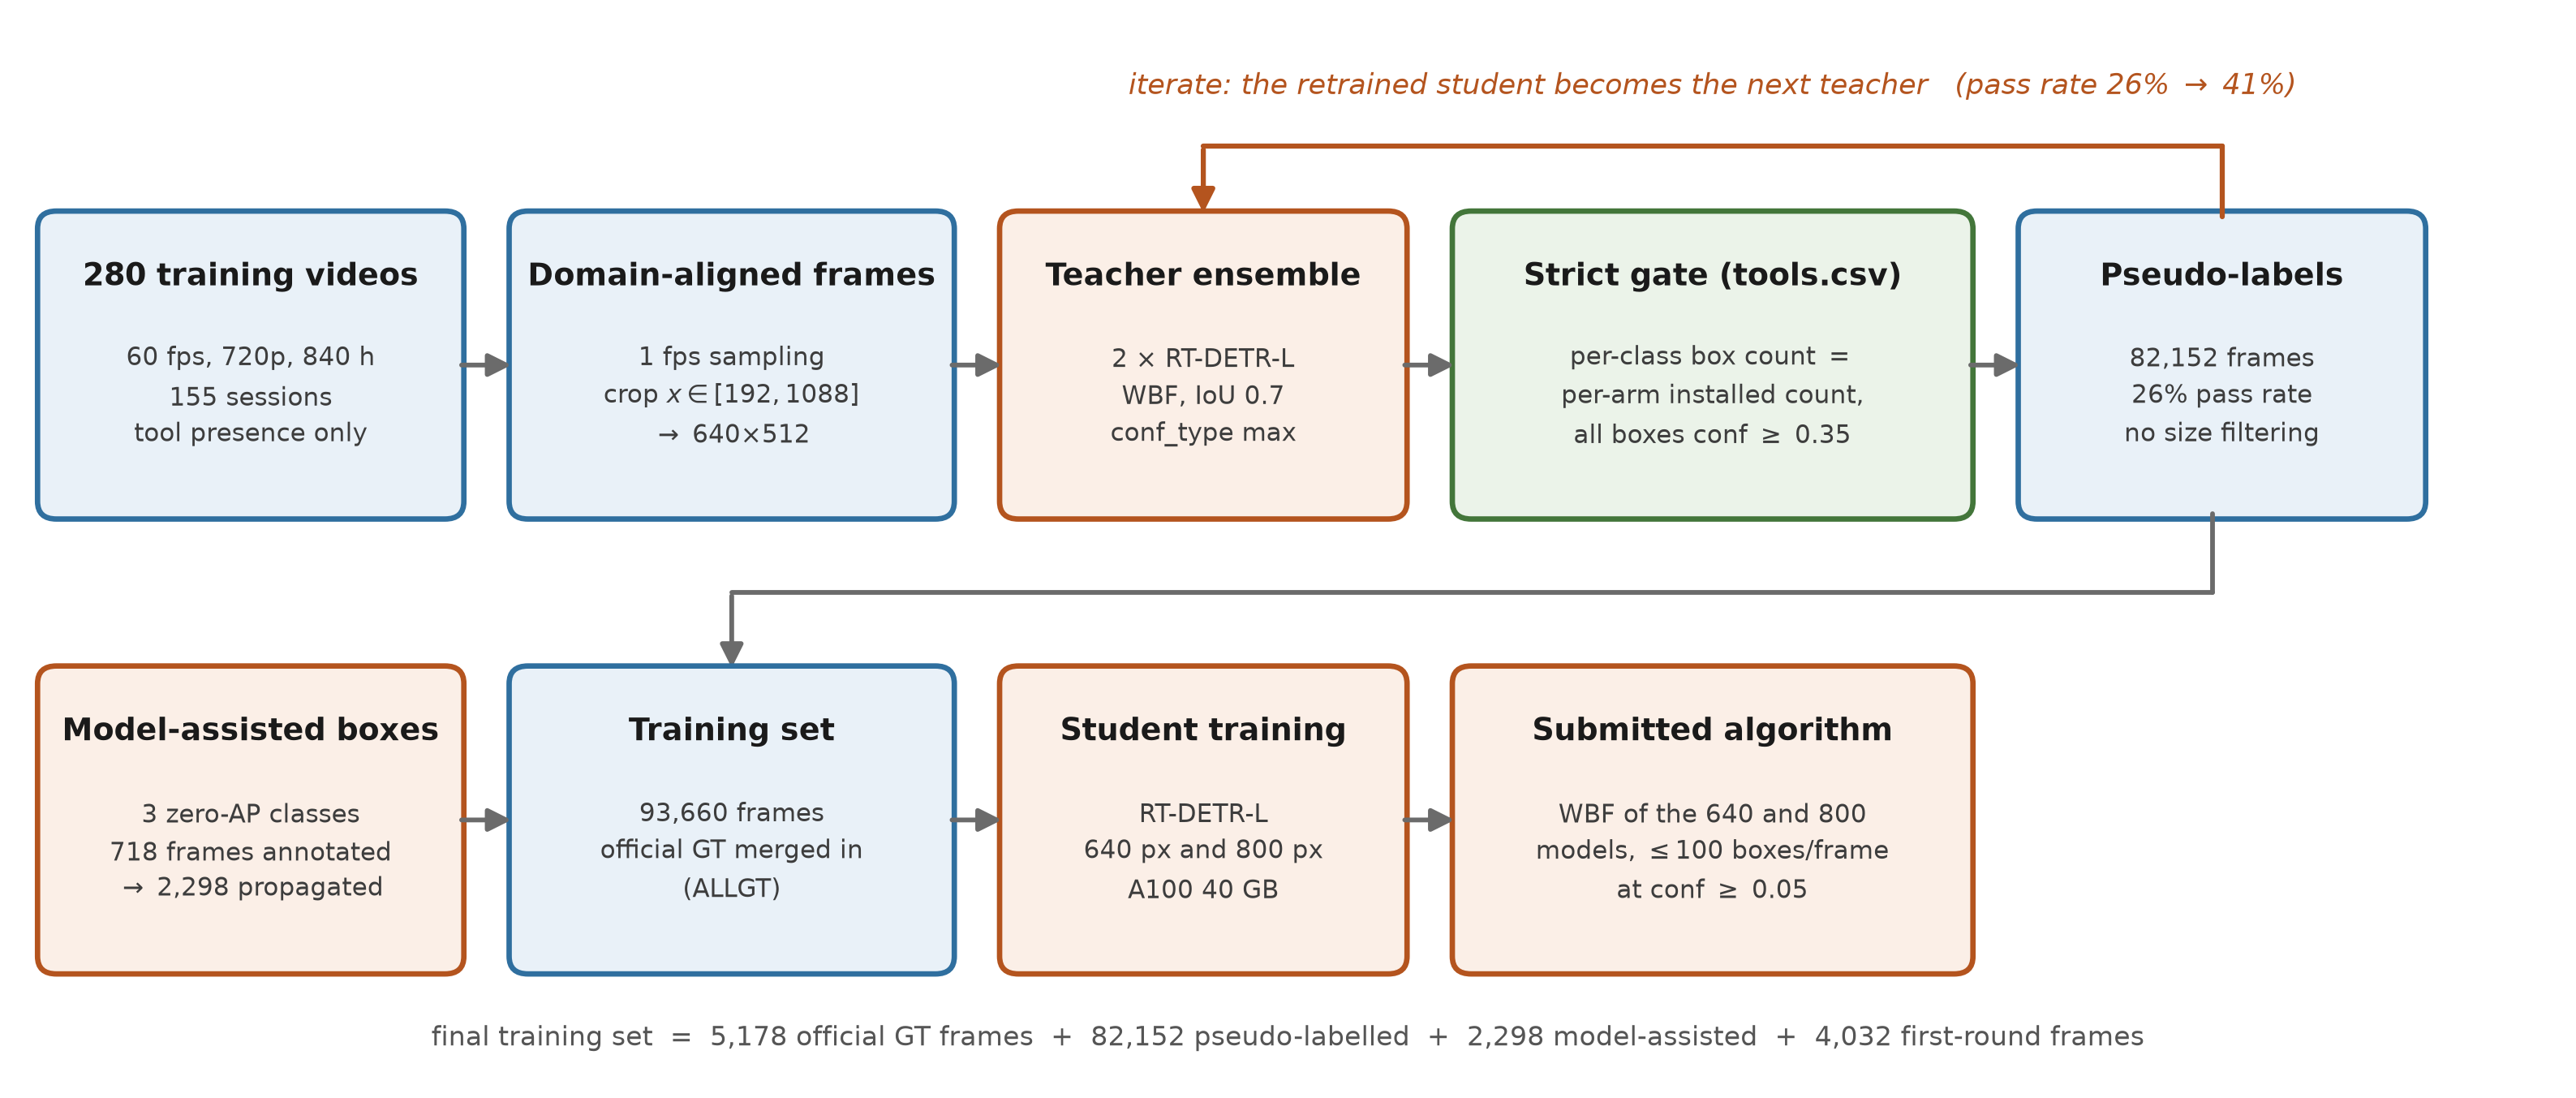
\includegraphics{TeamDocs2026/APC_TDC/figure1.png}}
\caption{Category~1 pipeline. Tool-presence labels act as an external gate on a teacher
ensemble; the accepted frames train a student that becomes the next teacher.}
\label{fig:APC_TDC_pipeline}
\end{center}
\end{figure}

\noindent\textbf{Domain alignment.} Public validation frames are $640\times512$ crops of the
$1280\times720$ feed. We reproduce that transform on training frames (crop $x\in[192,1088]$ at
full height, resize to $640\times512$) so pseudo-labelling, training and inference share one
geometry.

\medskip
\noindent\textbf{Weak labels.} We parse \texttt{tools.csv} per robot arm into the multiset of tools
installed at every second, resolving overlaps on one arm in favour of the shorter
interval and expanding labels across video parts.

\medskip
\noindent\textbf{Pseudo-labelling.} A teacher ensemble of two RT-DETR-L~\cite{APC_TDC_Zhao2024}
models predicts on every extracted frame; we fuse the predictions with weighted box fusion
(WBF, IoU $0.7$, \texttt{conf\_type} max)~\cite{APC_TDC_Solovyev2021}. We keep boxes with
confidence $\geq 0.20$ whose class appears in the installed multiset, drop boxes centred in
the da~Vinci interface banners, and drop whole frames in which two different classes share a
box (IoU $>0.7$). A frame is accepted only if the per-class box count equals the installed
count exactly and every kept box has confidence $\geq 0.35$. We apply \emph{no} box-size
filter: an earlier variant clipping box areas to the 2nd--98th percentile removed the near-
and far-field scale samples the detector needs and reduced AP75.

\medskip
\noindent\textbf{Iteration.} Retraining the teacher on its own accepted output raised the
acceptance rate from $26\%$ to $41\%$ and the pool from 82k to 142k frames. Iterative
pseudo-labelling converges here because \texttt{tools.csv} is an external, model-independent
filter.

\medskip
\noindent\textbf{Background-collapse failure.} Prograsp forceps, stapler and tip-up grasper were
initially dropped from the pseudo-label targets while their images were kept, teaching the
detector to treat visible instances as background: 65,182 of 149,569 frames listed one of them
as installed but carried no box, against 711 positive prograsp boxes. Deleting those frames
raised held-out detection of prograsp and stapler from $0.000$ to $0.255$ and $0.265$.

\medskip
\noindent\textbf{Inference.} The submitted container runs the 640 and 800 models and fuses
their per-frame detections with WBF, emitting at most 100 boxes per frame at confidence
$\geq 0.05$ with true confidence values. A wall-clock guard falls back to the
single 640 model if the projected runtime exceeds the per-case limit.

\medskip
\noindent\textbf{Category 2.} We classify each question into one of six types from the position of
its auxiliary verb and wh-word, then emit a templated sentence: BERTScore against
short reference answers rewards matching the expected answer \emph{form}. Yes/no polarity for
five high-recall tools is decided visually by our C1 detector over 15 sampled frames; the rest
fall back to a prior estimated from 30-second windows of
\texttt{tools.csv}.

\subsubsection{Model Training}

All detectors are RT-DETR-L (Ultralytics 8.4.137) initialised from COCO-pretrained weights and
trained on one NVIDIA A100 SXM4 40\,GB. We set the optimizer explicitly to AdamW
($\mathrm{lr}_0 = 5.56\times10^{-4}$, $\mathrm{lr}_f = 0.01$, momentum $0.9$, weight decay
$5\times10^{-4}$, \texttt{warmup\_bias\_lr} $=0$): Ultralytics silently switches
\texttt{optimizer=auto} to MuSGD at lr $0.01$ above 10{,}000 iterations, which would have changed
the recipe as the dataset grew. The submitted models use 16 epochs,
\texttt{close\_mosaic} 6, batch 24 at 640 (5.8\,h) and batch 20 at 800 (8.0\,h), with default
mosaic, scale and flip augmentation. The final training set is 93,660 frames. For ablations we
held official validation videos 1 and 7 out of the student; for the submitted
models we merged all annotated official videos into training and submit \texttt{last.pt}.

\subsubsection{Preliminary Performance}

Table~\ref{tab:APC_TDC_results} lists our official scores; data scale-up produced the
largest single gain. On the Final set, routing the four never-detected classes to a separate
model was worth $+0.0003$, while 800-pixel training with cross-model fusion was worth
$+0.0100$.

\begin{table}[!ht]
\begin{center}
\begin{tabular}{llr}
\toprule
Phase & Configuration & mAP \\
\midrule
C1 Preliminary & official validation videos only & 0.4372 \\
C1 Preliminary & domain-aligned strict pseudo-labels & 0.4464 \\
C1 Preliminary & pseudo-label source 20 $\rightarrow$ 280 videos & 0.5059 \\
\midrule
C1 Final & single model, 640 & 0.4830 \\
C1 Final & \, $+$ separate model for four zero-AP classes & 0.4833 \\
C1 Final & \, $+$ WBF of the 640 and 800 models & \textbf{0.4930} \\
\midrule
C2 Final & echo templates & 0.5833 \\
C2 Final & \, $+$ question-type routing fix & 0.6067 \\
C2 Final & \, $+$ visual yes/no polarity & \textbf{0.6191} \\
\bottomrule
\end{tabular}
\caption{Official scores. C1 is mAP@[.5:.95] averaged over videos; C2 is BERTScore-F1.}
\label{tab:APC_TDC_results}
\end{center}
\end{table}

In paired ablations on a student hold-out (official videos 1 and 7), 800-pixel
training gave $+0.0131$ mean mAP and $+0.0275$ AP75, and cross-model WBF gave $+0.0166$ and
$+0.0376$; both gains sit at high IoU, i.e.\ they tighten boxes rather than find more tools. What did not work: 39 inference-time variants had a ceiling of $+0.005$; ten
temporal post-processing variants were all negative; fine-tuning on official ground truth alone was worse
than mixed training, returning the model to the scale prior of five videos.

\medskip
\noindent\textbf{Limitations.} These ablations isolate the student, not the pipeline: the
teacher had seen the held-out videos, so absolute values are optimistic and only paired
differences should be read. We also saw a proxy metric invert: tool-presence set-F1 on 2,820
unseen frames rose from $0.578$ to $0.819$ for a relabelling scheme that was $-0.0127$ on
official-protocol mAP. Session-level splits and a
small human-annotated box set for the rare classes are the next steps.

\medskip
\noindent\textbf{Disclosure.} No external datasets were used. Bounding boxes for the three
never-detected classes were annotated with a large language model (Claude Opus~5) on 718
frames and expanded to 2,298 training frames by template matching ($2.5\%$ of the
training set); the annotation protocol and code are in our repository and the label
files are available to the organizers on request. A variant that read the da~Vinci
interface with EasyOCR to gate pseudo-labels at training time only was evaluated but is not
part of the submitted model.
